% mnras_template.tex 
%
% LaTeX template for creating an MNRAS paper
%
% v3.0 released 14 May 2015
% (version numbers match those of mnras.cls)
%
% Copyright (C) Royal Astronomical Society 2015
% Authors:
% Keith T. Smith (Royal Astronomical Society)

% Change log
%
% v3.0 May 2015
%    Renamed to match the new package name
%    Version number matches mnras.cls
%    A few minor tweaks to wording
% v1.0 September 2013
%    Beta testing only - never publicly released
%    First version: a simple (ish) template for creating an MNRAS paper

%%%%%%%%%%%%%%%%%%%%%%%%%%%%%%%%%%%%%%%%%%%%%%%%%%
% Basic setup. Most papers should leave these options alone.
\documentclass[fleqn,usenatbib,useAMS]{mnras}

% MNRAS is set in Times font. If you don't have this installed (most LaTeX
% installations will be fine) or prefer the old Computer Modern fonts, comment
% out the following line
\usepackage{newtxtext,newtxmath}
% Depending on your LaTeX fonts installation, you might get better results with one of these:
%\usepackage{mathptmx}
%\usepackage{txfonts}

% Use vector fonts, so it zooms properly in on-screen viewing software
% Don't change these lines unless you know what you are doing
\usepackage[T1]{fontenc}

% Allow "Thomas van Noord" and "Simon de Laguarde" and alike to be sorted by "N" and "L" etc. in the bibliography.
% Write the name in the bibliography as "\VAN{Noord}{Van}{van} Noord, Thomas"
\DeclareRobustCommand{\VAN}[3]{#2}
\let\VANthebibliography\thebibliography
\def\thebibliography{\DeclareRobustCommand{\VAN}[3]{##3}\VANthebibliography}


%%%%% AUTHORS - PLACE YOUR OWN PACKAGES HERE %%%%%

% Only include extra packages if you really need them. Common packages are:
\usepackage{graphicx}	% Including figure files
\usepackage{amsmath}	% Advanced maths commands
%% \usepackage{amssymb}	% Extra maths symbols

%%%%%%%%%%%%%%%%%%%%%%%%%%%%%%%%%%%%%%%%%%%%%%%%%%

%%%%% AUTHORS - PLACE YOUR OWN COMMANDS HERE %%%%%

% Please keep new commands to a minimum, and use \newcommand not \def to avoid
% overwriting existing commands. Example:
%\newcommand{\pcm}{\,cm$^{-2}$}	% per cm-squared

%%%%%%%%%%%%%%%%%%%%%%%%%%%%%%%%%%%%%%%%%%%%%%%%%%

%%%%%%%%%%%%%%%%%%% TITLE PAGE %%%%%%%%%%%%%%%%%%%

% Title of the paper, and the short title which is used in the headers.
% Keep the title short and informative.

\title[High-resolution ALMA observations of V4046\,Sgr]{High-resolution ALMA observations of V4046\,Sgr: a circumbinary disc with a thin ring}

% The list of authors, and the short list which is used in the headers.
% If you need two or more lines of authors, add an extra line using \newauthor
\author[R. Martinez Brunner et al.]{Rafael Martinez--Brunner,$^{1}$
\thanks{E-mail: rmartinezbrunner@gmail.com}
Simon Casassus,$^{1}$
Sebasti\'an P\'erez,$^{2}$
Antonio Hales,$^{3,4}$
Philipp Weber, $^{1,2}$ \newauthor
Miguel Carcamo,$^{5,6}$
Carla Arce-Tord,$^{1}$
Lucas Cieza,$^{7}$
Antonio Garufi,$^{8}$
Sebasti\'an Marino,$^{9}$
Alice Zurlo$^{7,10,11}$
\\
% List of institutions
$^{1}$Departamento de Astronom\'ia, Universidad de Chile, Casilla 36-D, Santiago, Chile\\
$^{2}$Departamento de F\'isica, Universidad de Santiago de Chile, Av. Ecuador 3659, Santiago\\
$^{3}$Joint ALMA Observatory, Avenida Alonso de C\'ordova 3107, Vitacura 7630355, Santiago, Chile \\
$^{4}$National Radio Astronomy Observatory, 520 Edgemont Road, Charlottesville, VA 22903-2475, United States of America \\
$^{5}$Departamento de Ingenier\'ia Inform´atica, Universidad de Santiago de Chile, Av. Ecuador, 3659, Santiago, Chile\\
$^{6}$Jodrell Bank Centre for Astrophysics, Alan Turing Building, Department of Physics and Astronomy, Alan Turing Building,\\ University of Manchester, Oxford Road, Manchester, M13 9PL, UK \\
$^{7}$N\'ucleo de Astronom\'ia, Facultad de Ingenier\'ia y Ciencias, Universidad Diego Portales, Av. Ejercito 441, Santiago, Chile\\
$^{8}$INAF, Osservatorio Astrofisico di Arcetri, Largo Enrico Fermi 5, I-50125, Firenze, Italy\\
$^{9}$Institute of Astronomy, University of Cambridge, Madingley Road, Cambridge CB3 0HA, UK\\
$^{10}$Escuela de Ingenier\'ia Industrial, Facultad de Ingenier\'ia y Ciencias, Universidad Diego Portales, Av. Ejercito 441, Santiago, Chile \\
$^{11}$Aix Marseille Universit\'e, CNRS, LAM - Laboratoire d'Astrophysique de Marseille, UMR 7326, 13388, Marseille, France  \\
}

% These dates will be filled out by the publisher
\date{Accepted XXX. Received YYY; in original form ZZZ}

% Enter the current year, for the copyright statements etc.
\pubyear{2021}

% Don't change these lines
\begin{document}
\label{firstpage}
\pagerange{\pageref{firstpage}--\pageref{lastpage}}
\maketitle

% Abstract of the paper
\begin{abstract}
    The nearby V4046\,Sgr spectroscopic binary hosts a gas-rich disc known for its wide cavity and dusty ring. We present high resolution ($\sim$20--50\,mas) ALMA observations of the 1.3\,mm continuum of V4046\,Sgr which, combined with SPHERE--IRDIS polarized images and well-sampled spectral energy distribution (SED), allow us to propose a physical model using radiative transfer (RT) predictions. The new ALMA data reveal a very thin ring at a radius of 13.15$\pm$0.26\,au (Ring13), with a marginally resolved radial width of 2.46$\pm$0.56\,au. Ring13 is surrounded by a $\sim$10\,au-wide gap, and it is flanked by a very mm-bright outer ring (Ring24) with a sharp inner edge at 24\,au. Between 25\,au and $\sim$35\,au the brightness of Ring24 is relatively flat and then breaks into a steeper tail that reaches out to $\sim$60\,au. In order to reproduce the SED, the model that we propose requires an inner ring at $\sim$5\,au (Ring5) composed mainly of small dust grains, hiding under the IRDIS coronagraph, and surrounding an inner circumbinary disc. The surprisingly thin Ring13 is nonetheless roughly 4 times wider than its expected vertical extent. The strong near-far disc asymmetry at 1.65\,$\micron$ points at a very forward-scattering phase function, and requires grain radii of no less than 0.4\,$\micron$. The previously reported scattered-light shadow of the secondary star is also reproduced by our physical model.
\end{abstract}

% Select between one and six entries from the list of approved keywords.
% Don't make up new ones.
\begin{keywords}
 protoplanetary discs -- submillimetre: planetary systems -- radiative transfer
\end{keywords}

%%%%%%%%%%%%%%%%%%%%%%%%%%%%%%%%%%%%%%%%%%%%%%%%%%

%%%%%%%%%%%%%%%%% BODY OF PAPER %%%%%%%%%%%%%%%%%%

\section{Introduction} \label{sec:Introduction}

Recent observations of young circumstellar discs have transformed current knowledge of planet formation. The focus of resolved imaging with the Atacama Large Millimeter/submillimeter Array (ALMA) or with the current generation of high-contrast cameras has mainly been towards the brighter sources \citep[e.g.][]{2020ARA&A..58..483A}. It is to address this bias that the programme called ``Discs Around T Tauri Stars with SPHERE'' (DARTTS-S) collected differential polarization imaging (DPI) data secured with the Spectro-Polarimeter High-contrast Exoplanet REsearch \citep[SPHERE][]{2019A&A...631A.155B} in a total of 29 solar-type stars \citep[][]{Avenhaus_2018,Garufi2020}. The sample is not biased towards exceptionally bright and large discs. The DARTTS observations revealed diverse structures and morphologies in the scattering surface of these discs. This article on V4046 Sagittarii (Sgr) is the first installment of a companion programme, the DARTTS survey with ALMA (DARTTS-A), which will present millimetre observations of nine protoplanetary discs previously imaged in polarized scattered light in DARTTS-S.

Disc structures can be explored by means of comparing millimetre continuum and scattered-light images. These observations allow us to see the distribution of different populations of dust particles: while ALMA traces the millimetre-sized grains settled in the mid-plane of the disc, scattered-light imaging accounts for photons reflected off micron-sized dust at the disc surface layer, high above the mid-plane. Therefore, the comparison of both allows to trace the dynamics present at different vertical heights in the disc.

V4046\,Sgr is a double-lined spectroscopic binary of K-type stars (K5 and K7) with very similar masses of 0.90$\pm$0.05\,M$_{\sun}$ and 0.85$\pm$0.04\,M$_{\sun}$ \citep{Rosenfeld_2012}, on a close ($a \approx 0.041$\,au), circular ($e\leq0.01$) orbit, with an orbital period of 2.42 days \citep{2000IAUS..200P..28Q}. It is a member of the $\beta$ Pictoris moving group \citep{Zuckerman_2004}, with an estimated age of 18.5$^{+2.0}_{-2.4}$\,Myr \citep{2020A&A...642A.179M}, and its distance is 71.48$\pm$0.11\,pc \citep{gaiacollaboration2020gaia}. V4046\,Sgr hosts a massive ($\sim$0.1\,M$_{\sun}$) circumbinary disc extending to $\sim$300\,au \citep{Rosenfeld_2013, Rodriguez_2010}, rich in diverse molecular lines \citep{Kastner_2018}.

From previous analysis of radio wavelength observations taken with Sub-millimeter Array (SMA) \citep{Rosenfeld_2013} and subsequently with ALMA \citep{Guzman_2017,Huang_2017,Bergner_2018,Kastner_2018}, it was detected that the millimetre dust configuration of the circumbinary disc had a large inner hole of $\sim$30\,au, featuring a narrow ring centred around 37\,au that accounted for most of the dust mass. By using DPI in the J- and H-band, \citet{Avenhaus_2018} confirmed the double-ring morphology previously presented in \citet{Rapson_2015}, where the observed brightness presented a $\sim$10\,au-wide inner cavity, a narrow ring at $\sim$14\,au and the outer ring centred at $\sim$27\,au.

The suggestion of a parametric model that simultaneously fits the NIR scattered-light and millimetre continuum brightness is challenging and has been attempted in only few previous studies \citep[e.g.][]{Dong_2018,2019MNRAS.486..304B, Ru_z_Rodr_guez_2019}. A successful model can serve as a convenient sample to link the observations to the structure of the underlying dust density distribution.

In this paper we present new observations of the continuum emission at 1.3 mm of V4046 Sgr which reveal previously undiscovered structures. This work also aims to reproduce the observations of the protoplanetary disc around V4046\,Sgr with a 3D model using as guidance previous NIR images, the spectral energy distribution (SED) and a new high definition 1.3\,mm continuum ALMA image, as a way to throw light on its complex structure and the processes that are occurring in it.

The details of the observations taken into account are described in Section~\ref{sec:Observations}. The parametric model is presented in Section~\ref{sec:model}, the results are discussed in Section~\ref{sec:results} and in Section~\ref{sec:Conclusions} we present our conclusions.

\section{Observations} \label{sec:Observations}
\subsection{ALMA}  \label{subsec:ALMA}

New ALMA observations of V4046\,Sgr were obtained in 2017 as part of the Cycle 5 program 2017.1.01167.S (PI: S. Perez). The observations acquired simultaneously the 1.3\,mm continuum and the J = 2$-$1 line of $^{12}$CO (i.e. with a band 6 211-275\,GHz correlator setup). The ALMA array was in its C43-8 configuration, with baselines ranging from 92 to 8548\,m which translate into a synthesized beam of $0\farcs062 \,\times \, 0\farcs055$, in natural weights. Here we focus on the continuum observations only. The line data will be presented in the main DARTTS-A paper.

Image synthesis of the ALMA continuum was performed with the {\tt uvmem} package \citep{2006ApJ...639..951C, 2018A&C....22...16C}, which fits a non-parametric model image $I^m_j$ to the data by comparing the observed and model visibilities, $V^\circ_k$ and $V^m_k$, using a least-squares figure of merit $L$:
\begin{equation}
  L = \sum_{k=1}^N \omega_k  |V^\circ_k - V^m_k|^2 + \lambda S,
\end{equation}
where $\omega_k$ are the visibility weights and $\lambda$ is a dimensionless parameter that controls the relative importance of the regularization term $S$.

The chosen regularization term $S$ for this case was the standard image entropy, or
\begin{equation}
S = \sum_{j=1}^M \frac{I_j^m}{M} \ln\left(\frac{I_j^m}{M}\right),
\end{equation}
where $M$ is the default pixel intensity value and is set to $10^{-3}$ times the theoretical noise of the dirty map (as inferred from the visibility weights $\omega_k$). Here we set $\lambda = 0.01$. Similar applications of {\tt uvmem} in the context of protoplanetary discs can be found, for example, in \citet{Casassus2013Natur, 2018MNRAS.477.5104C, Casassus2019MNRAS.483.3278C, Perez2019AJ....158...15P} and in \citet{2020ApJ...889L..24P} using long baseline data. An advantage of {\tt uvmem} compared to more traditional imaging strategies, such as provided by the {\tt tclean} task in CASA, is that the effective angular resolution of the model image is $\sim$3 times finer than the natural weights clean beam \citep[][]{2018A&C....22...16C}, giving us a new approximate {\tt uvmem} resolution of $\sim0\farcs021 \,\times \,\sim0\farcs018$. This angular resolution is comparable to uniform or super-uniform weights in {\tt tclean}, but it preserves the natural-weights point-source sensitivity.

The resulting {\tt uvmem} image shown in the top right panel of Fig.~\ref{fig:images_vs_simulated} exhibits previously unseen substructure of the disc. This image reveals that the disc features two rings of large dust grains with a broad gap between them, i.e. Ring13 at 13\,au and Ring24 starting at 24\,au. The wide and bright Ring24 reaches its peak intensity at $\sim$30\,au, beyond which it drops steeply before breaking at $\sim$35\,au into a shallow tail. While this is the first observation of Ring13, \citet{Ru_z_Rodr_guez_2019} did anticipate its existence as their ALMA continuum image showed a distinct excess between $\sim$10 and 17\,au. The {\tt uvmem} map has a resolution of 21$\times$18\,mas and an RMS noise of 26$\micron$Jy per resolution beam, at a frequency of 237 GHz.

Ring13 is surprisingly narrow and seems to be off-centred relative to the Gaia stellar position, at the origin of coordinates in Fig.~\ref{fig:images_vs_simulated}. We determined the ring's centre and orientation by minimising the dispersion of the disc radial profiles from 6\,au to 19\,au, by using the {\tt MPolarMaps} package described in Casassus et al. (2021, in prep). The resulting disc orientation is set at a position angle (PA) of 77.31$\pm$0.03\,$\degr$ (east of north), with an inclination of 32.96$\pm$0.02\,$\degr$, and the optimal ring centre is at $\Delta \alpha = -4\pm0.02$\,mas $\Delta \delta = 13\pm0.05$\,mas relative to the Gaia position of the stars. The offset of the center of the cavity and the nominal stellar positions is entirely consistent with a pointing error, since the pointing accuracy of ALMA is $\sim$5\,mas for the signal to noise ratio of our image (calculated using the ALMA Technical Handbook).

The ring width can be measured in polar coordinates by fitting 1-D Gaussians at each azimuth, thus obtaining a width and centroid. The top panel of Fig.~\ref{fig:polarring}) shows the positions of the obtained centroids and widths over the polar decomposition of the ALMA image. On average, we obtained a FWHM of 2.83$\pm$0.25\,au, and a stellocentric radius of 13.15$\pm$0.42\,au. As the {\tt uvmem} model image has an approximate {\tt uvmem} beam of $\sim0\farcs021 \,\times \,\sim0\farcs018$, we see that Ring13 is marginally resolved. After subtraction of the {\tt uvmem} beam, the ring width is $\sim$2.46$\pm$0.40\,au.

In a second optimization of the disc orientation, but this time aiming for Ring24 with a radial domain from 20\,au to 70\,au, we obtained a PA of 76.86$\pm$0.02\,$\degr$, with an inclination of 33.92$\pm$0.01\,$\degr$ and a centre at $\Delta \alpha = 2\pm0.02$\,mas $\Delta \delta = 12\pm0.02$\,mas relative to the stars. We see that both Ring13 and Ring24 share a very similar orientation and centre, given the errors. However, quite likely due to the joint effect of all these small differences, we can see that there are some hints for a somewhat different orientation. This is summarised in the second panel of Fig.~\ref{fig:polarring}, where it shows the centroids of the Gaussian fitting at each azimuth for both optimization. The curve that follows these fitted centroids for each of the optimizations goes almost entirely within the errors of the other one, leaving the window open to the discussion of if this differences are just a consequence of the pointing error or are they a real notable feature of the disc.

Interestingly, the ALMA image also detects faint 1.3\,mm continuum emission near the stellar positions (see the inset in Fig.~\ref{fig:images_vs_simulated}). Since this faint central emission is larger than the angular resolution, it is probably stemming from thermal emission from large dust grains rather than directly from the stars. The main blob of this dust structure is at estimated distance of only $0\farcs012\pm0\farcs002$, or $\sim$0.85$\pm$0.14\,au from the binary system, and, estimating its form as a Gaussian ellipse, it has a mean FWHM of $\sim$1.43\,au. \citet{Francis_2020} also did some measurements of this central emission by assuming a power--law profile for an inner disk that goes from 0.1 to 4\,au, and has a total dust mass of 0.013$\pm$0.002\,M$_{\earth}$. They stated that the inner radius of the disk is well beyond the sublimation radius as the system shows a low--NIR excess but a clear millimetre emission.

%If this feature is caused by the presence of millimetre-sized dust, assuming optically thin emission, i.e. following
%\begin{multline}
%    \label{optically_thin_equation}
%      M_{blob} = 0.03 M_{\sun} \left(\frac{F}{1\,\mathrm{Jy}}\right) \left(\frac{d}{100\,\mathrm{pc}}\right)^2 \left(\frac{\lambda}{1.3\,\mathrm{mm}}\right)^3 
%      \\
 %     \left(\frac{50\,\mathrm{K}}{T}\right)    %\left(\frac{0.02\,\mathrm{cm^2/g}}{\kappa_{1.3\,\mathrm{mm}}}\right),
%\end{multline}
%where $F$ is the total flux of the blob, $d$ the distance of 71.4\,pc , $\lambda$ the wavelength, $\kappa_{1.3\,\mathrm{mm}}$ the opacity at 1.3\,mm and the temperature set at $T=500\,\mathrm{K}$. Then, its estimated mass would be around 0.12\,M$_{\earth}$.

\subsection{SPHERE--IRDIS}  \label{subsec:SPHERE}

V4046\,Sgr was observed in DPI mode with SPHERE--IRDIS on March 13, 2016 \citep[see][for details]{Avenhaus_2018}. Here we use a new reduction of the $H$ band data produced with the IRDAP pipeline \citep{2020A&A...633A..64V}, which can separate stellar and instrumental polarization. The polarized signal is consistent with the previous image in \citet{Avenhaus_2018}. The degree of linear polarization of the central and unresolved signal in V4046\,Sgr is only 0.13\%, with a systematic uncertainty of 0.05\% due to time-varying atmospheric conditions during the exposures. The angle of polarization is aligned with the disc major axis, as expected given that the target has an extinction of Av=0.0 \citep{2016ApJ...828...69M} and the entire polarization is dominated by circumstellar rather than inter-stellar material.

\begin{figure*}
  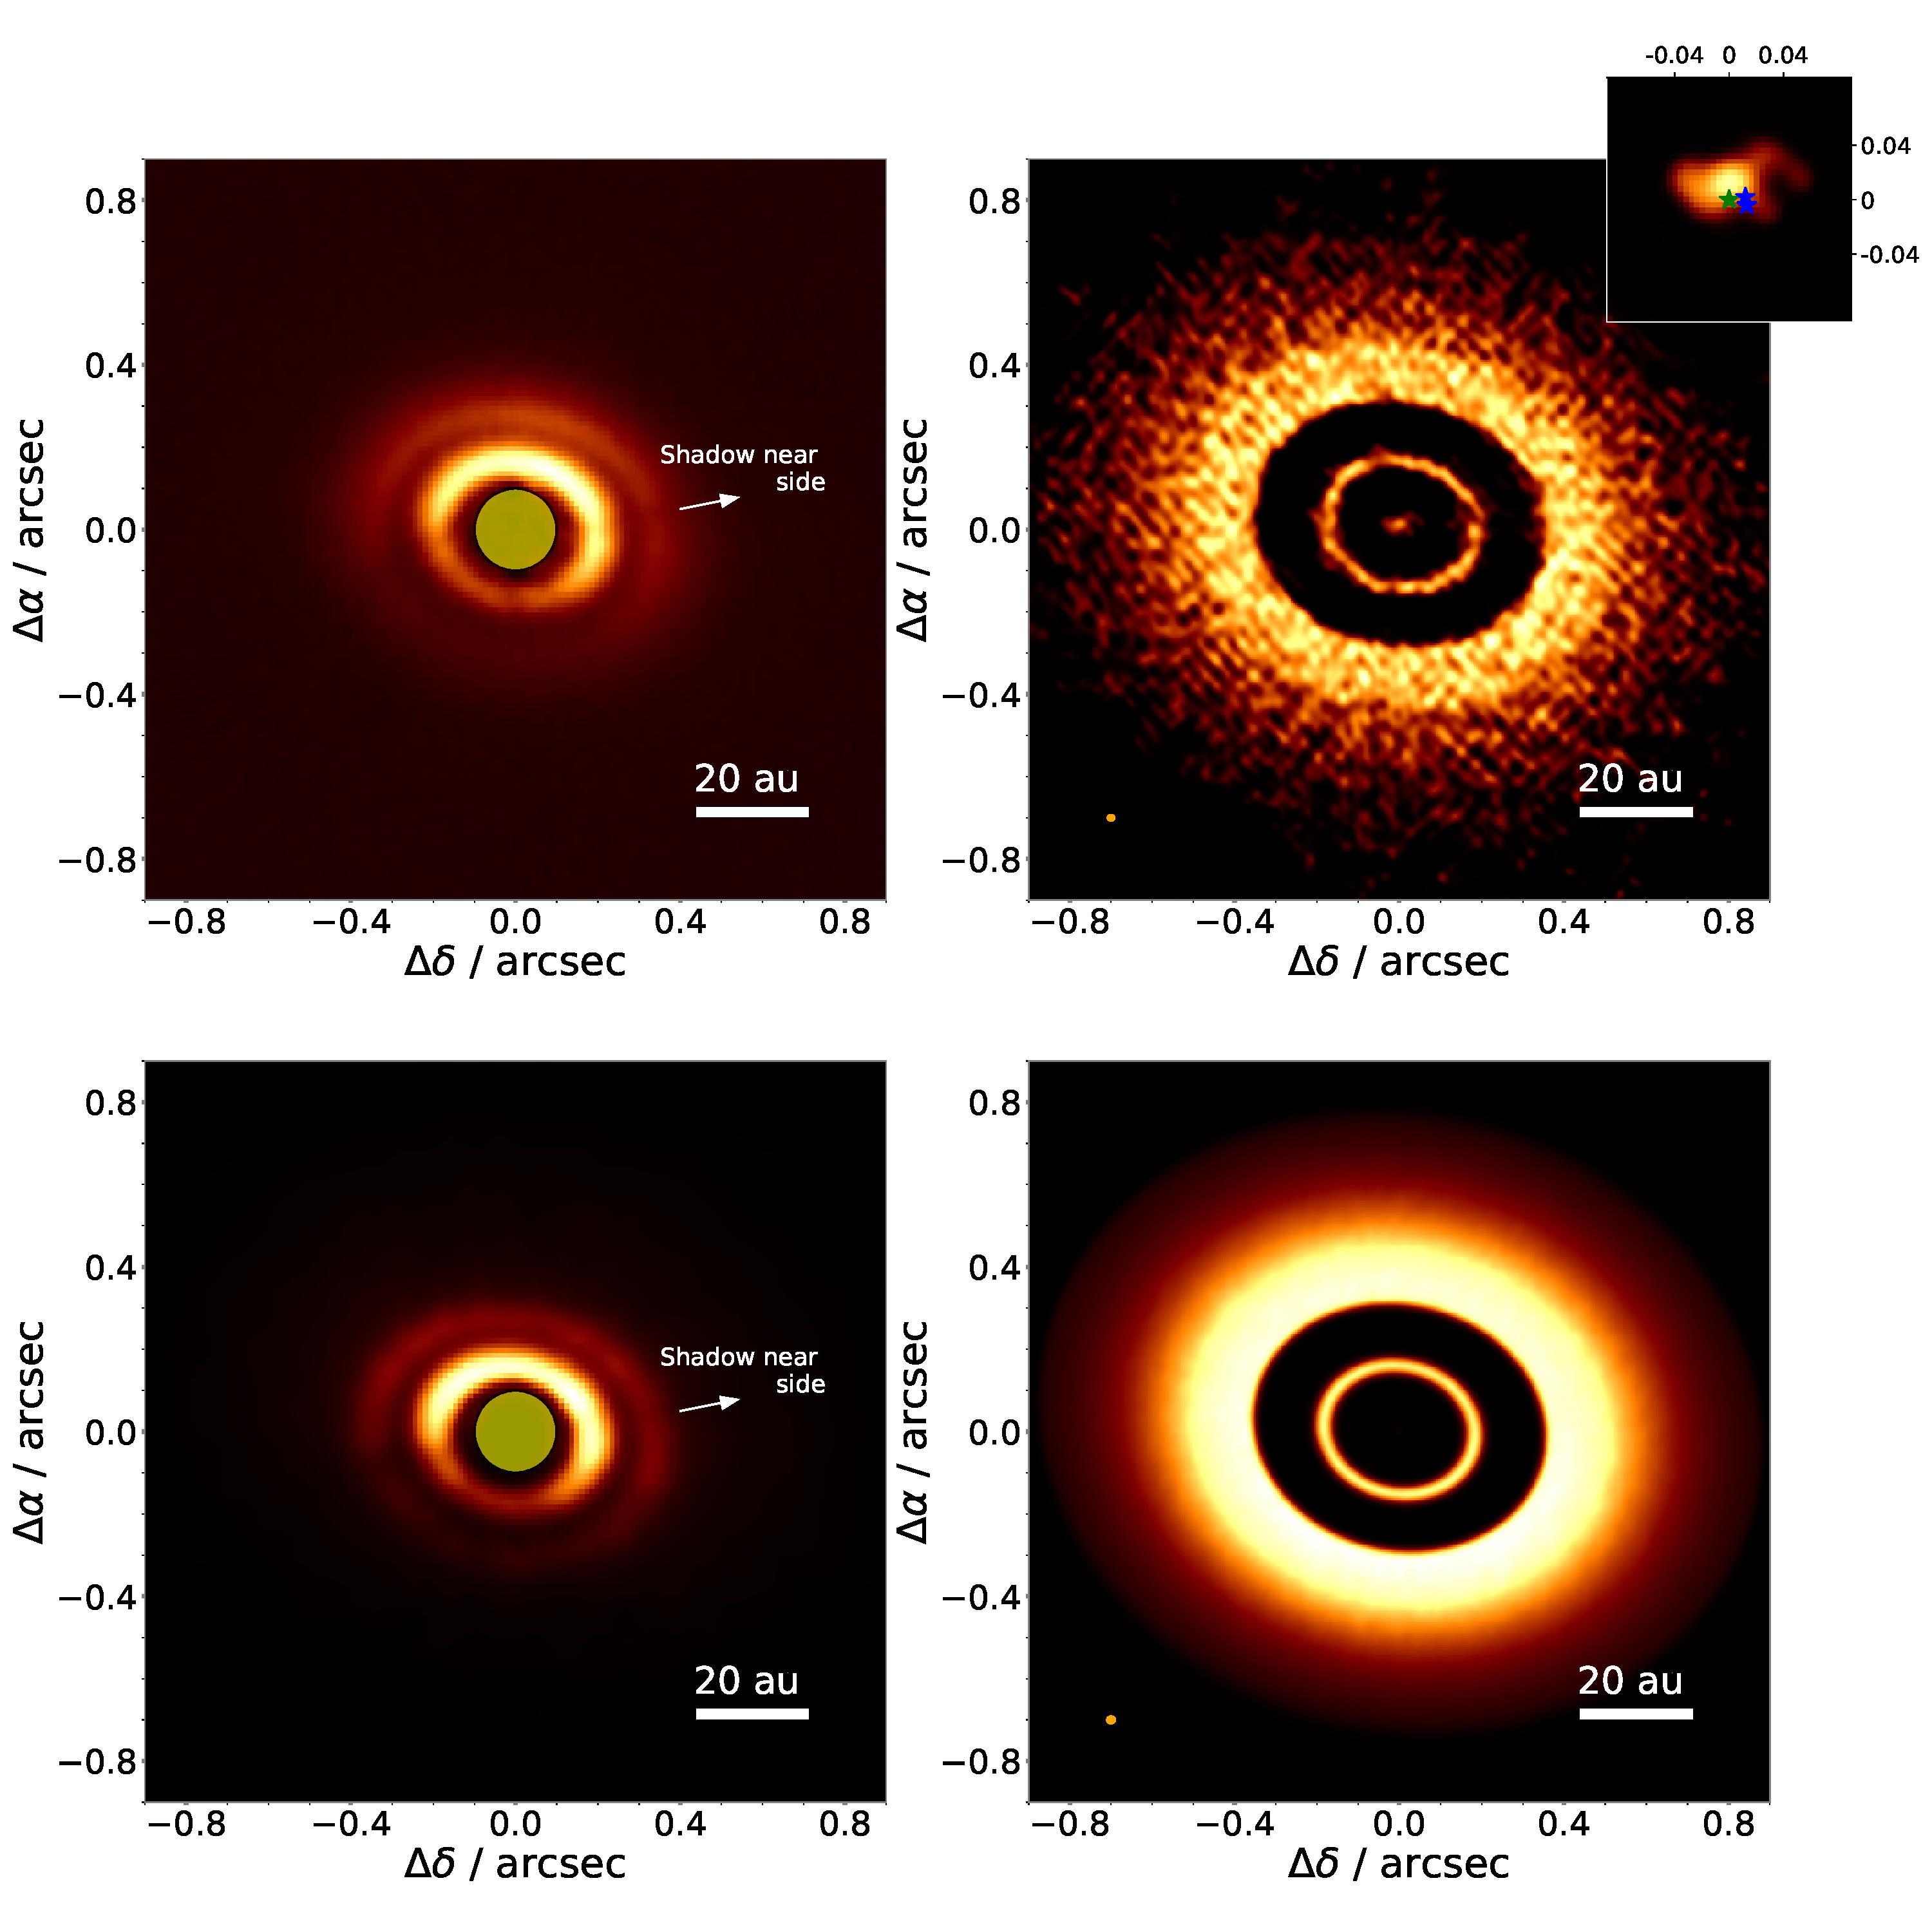
\includegraphics[width=\textwidth]{hot_two_E.pdf}
  \caption{Comparison of observations (top) and simulated images (bottom) at 1.65\,$\micron$ (left) and 1.3\,mm continuum (right) of the circumbinary disc orbiting V4046\,Sgr. \textit{Top left panel:} SPHERE--IRDIS \textit{H}-band image with a yellow filled circle that represents the N\_ALC\_YJH\_S coronagraph with a radius of $\sim0\farcs12$, or $\sim$8.6\,au at 71.48\,pc. \textit{Top right panel:} 1.3\,mm continuum {\tt uvmem} model image. The small orange ellipse shows an estimated {\tt uvmem} beam size ($\sim0\farcs021 \, \times \, \sim0\farcs018$). The inset zooms into the central emission, and the green star marks the center of the inner ring. \textit{Bottom left panel:} synthetic image at 1.65\,$\micron$. \textit{Bottom right panel:} synthetic image at 1.3\,mm convolved with the {\tt uvmem} beam. For all the images in the figure the colour scale is linear.}
  \label{fig:images_vs_simulated}
\end{figure*}

The scattered-light image in the top left panel of Fig.~\ref{fig:images_vs_simulated} also shows a double ring structure in the micron-sized dust distribution. The observed morphology presents an inner cavity of $\sim$10\,au in radius and two rings located at 14.10$\pm$0.01\,au, coincident with Ring13, and 24.62$\pm$0.08\,au, coincident with Ring24, with a small gap between them at $\sim$20\,au. The observed second ring matches the inner wall of the 1.3\,mm continuum emission outer ring \citep{Ru_z_Rodr_guez_2019}. Two other important features that are present in the image are: the near-far brightness asymmetry, and the shadows projected on the disc by the close binary system as they eclipse each other, discovered by \citet{dOrazi}.

The binary phase reported by \citet{dOrazi} in the scattered-light observation is at a PA of 265\,$\degr$, east of north. Using this measurement, the binary phase was calculated at the time of the ALMA observation at a PA of $\sim$80\,$\degr$. There is no hint of radio decrements in either Ring13 nor in Ring24 that would match shadowing at this PA. This could be explained by inefficient disc cooling compared to the speed of the illumination pattern \citep[see ][ for estimates of this cooling timescale]{Casassus2019MNRAS.486L..58C}.

\begin{figure}
    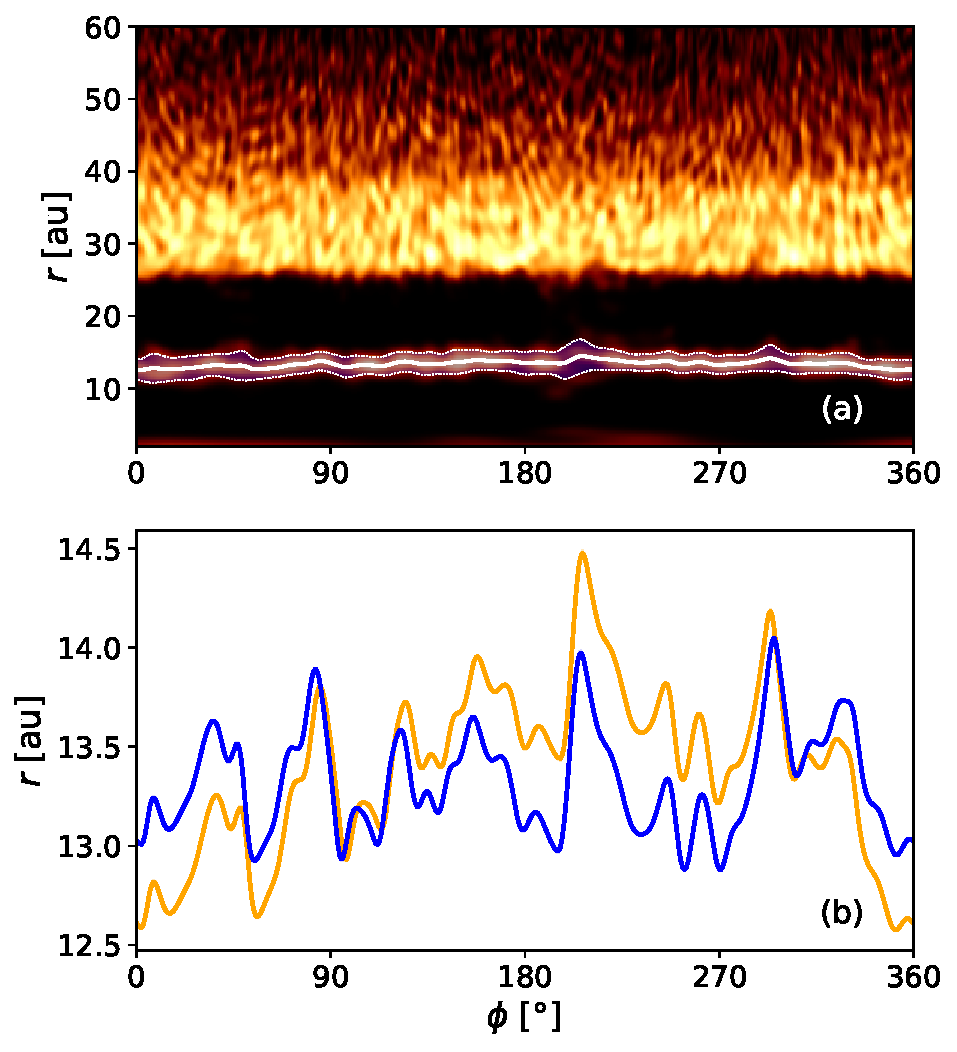
\includegraphics[width=\columnwidth]{polar_ring_aprox_and_diff_inner.pdf}
    \caption{{\bf (a)} Polar decomposition of the 1.3\,mm continuum image, using the orientation of Ring24. We trace Ring13 using the centroids (solid line) and width of radial Gaussian fits (blue region between the dotted lines). {\bf (b)} Centroid of Ring13, for two disc orientations: the orange line corresponds to the same trace as in (a), while the blue line is obtained for the inner ring orientation.}
    \label{fig:polarring}
\end{figure}

\subsection{Spectral energy distribution} \label{subsec:SED}

The observed SED was collected from data in the literature \citep{1988iras....7.....H, 1990A&A...234..230H, Jensen_97, 2000A&A...355L..27H, 2001KFNT...17..409K, 2003yCat.2246....0C, 2007PASJ...59S.369M, 2008PASP..120.1128O, 2010A&A...514A...1I, 2012yCat.2311....0C}, available online in \textsc{vizier}. We also used archival \textit{Spitzer} IRS spectroscopic data available in the CASSIS database \citep{Lebouteiller_2015} (see Fig.~\ref{fig:SED}). The SED describe the characteristic “dip” near 10 $\micron$, a common element of transition disc, as described by \citet{Rosenfeld_2013}. \citet{Jensen_97} concluded that these data matched that of a extended circumbinary disc truncated at $\sim$0.3\,au, as the interior would also be expected to be cleared by dynamical effects of the central binary \citep{Art_Lu}.

\begin{figure}
	\centering
	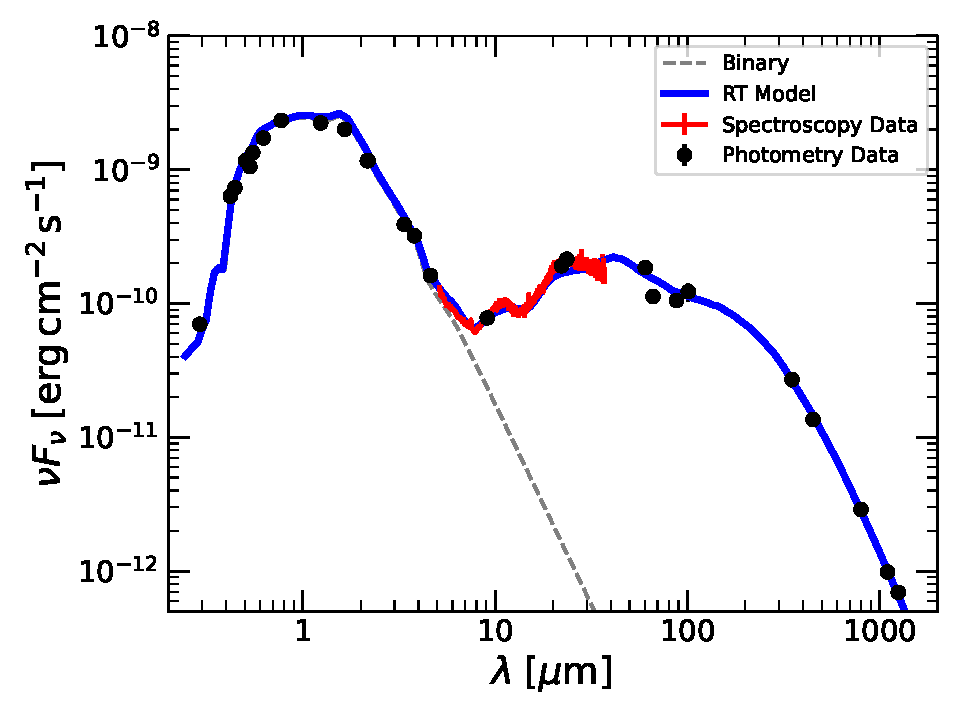
\includegraphics[width=\columnwidth]{SED_.pdf}
    \caption{The observed SED of V4046\,Sgr (black points and solid red curve) compared with the model (blue). The black points represent the measured photometry and the red line shows an archival \textit{Spitzer} IRS spectrum. The dashed silver curve shows the emission of the stellar photosphere model.}
    \label{fig:SED}
\end{figure}

\section{Parametric radiative transfer model} \label{sec:model}

The multi-frequency data can be interpreted in terms of a physical structure using radiative transfer predictions, for which we used the \textsc{radmc3d} package \citep[version 2.0,][]{Dullemond_2012}. The general framework of the parametric model that we developed is similar to that in \citet{2018MNRAS.477.5104C} for DoAr\,44, and the initial model values were inspired from those in \citet{Rosenfeld_2013}, \citet{Ru_z_Rodr_guez_2019} and \citet{2019ApJ...882..160Q}. Computing a high-resolution radiative transfer model that succeeds in the reproduction of multi-frequency imaging and the SED, is finding a solution to a highly degenerative problem, so obtaining an ideal model with a full parameter exploration requires a level of computation and time that exceeds our capabilities and the scope of this paper. Consequently, our approach was to find through trial and error a set of values for the parameters that closely fit the available data, and then, improve this fit by implementing one dimensional chi squared optimizations for some key parameters (more on this in sec.~\ref{sec:results}). The final structure of the parametric model is summarised in Fig.~\ref{fig:profiles}, where we show on the top panel surface density profiles for gas, large and small dust grains, and in the bottom panel the respective aspect ratio profile.

The stars were modeled using two Kurucz photosphere models \citep{1979ApJS...40....1K, 1997A&A...318..841C}, with T$_{\mathrm{eff},1} =$ 4350\,K, R$_{*,1} =$ 1.064\,R$_{\sun}$, M$_{*,1} =$ 0.90\,M$_{\sun}$ and T$_{\mathrm{eff},2} =$ 4060\,K, R$_{*,2} =$ 1.033\,R$_{\sun}$, M$_{*,2} =$ 0.85\,M$_{\sun}$, respectively and with an accretion rate of $\mathrm{log}(\,\dot{\mathrm{M}}/(\mathrm{M}_{\sun}\,\mathrm{yr^{-1}})) = -$9.3 for both cases to include excess UV due to stellar accretion \citep{10.1111/j.1365-2966.2011.19366.x}. The stars were placed at a mutual separation of 0.041\,au, so that their centre of mass coincides with the origin. Their PA was set to 250\,$\degr$, so that the secondary lies to the NW from the primary, thus casting the same shadow as observed by \citet{dOrazi}.

Reproducing the radial and vertical structure of the V4046\,Sgr disc turned out to be challenging. We built the model in terms of the gas distribution, and with two main dust populations: larger grains that are vertically settled and dominate the total dust mass, and a population of smaller grains that are uniformly mixed with the gas and reach higher regions above the mid-plane. And we also added a third dust population of large grains and with a tightly confined distribution and a special size range just to account for the central emission.

Assuming a three dimensional model in a cylindrical reference frame with coordinates ($r$, $\theta$, $z$), the gas density ($\rho_{\mathrm{gas}}$) distribution follows
\begin{equation}
  \rho_{\mathrm{gas}}(r,z) =\frac{\Sigma_{\mathrm{gas}}(r)}{\sqrt{2\pi} \, H(r)} \mathrm{exp}\left[-\frac{1}{2} \left(\frac{z}{H(r)}\right)^2\right],
\end{equation}
where $H(r)$ is the scale height profile and $\Sigma_{\mathrm{gas}}(r)$ is the gas surface density profile.

The parametric scale height profiles for the gas and for each dust population are 
\begin{equation}
    \label{scale}
  H(r)=\chi \, H_{\circ} \,\left( \frac{r}{r_{\circ}}\right)^{1+\psi(r)},
\end{equation}
where $H_\circ$ is the scale height at $r$ = $r_\circ$, $\psi$ is the flaring index and $\chi$ is a scaling factor (in the range $0-1$) that mimics dust settling. In hydrostatical equilibrium dust diffusion and settling are expected to balance each other, leading to a settling factor of $\chi = \sqrt{D_{\rm d}/(D_{\rm d} + St)}$ \citep{Dubrulle1995}. Here, $D_{\rm d}$ is a dimensionless parameter that informs about the level of diffusivity (it is typically assumed to be similar to the level of turbulence for the particle sizes regarded here \citep{2007Icar..192..588Y}. The Stokes number,
\begin{equation}
    {\rm St} := \frac{1}{2} \,\frac{\pi a \rho_{\rm mat}}{\Sigma_{\rm gas}}, 
\end{equation}
summarises a particle's dynamical behaviour in a given environment (where $\rho_{\rm mat}$ represents a dust particle's material density). By definition, the gas has no settling, and the small dust grains settling is negligible, so that $\chi_{\rm gas}=\chi_{\rm sd}=1$. As we do not know the level of diffusivity in the disc (this will be a topic of interest in Section~\ref{sec:results}), nor the exact value of $\Sigma_{\rm gas}$, we infer the scaling factor for large dust, $\chi_{\rm ld}$, from the width of Ring13. In the radial profile this ring is observed two to three times wider in the gas-tracing NIR than in the fluxes received from larger grains by ALMA. We assume that the same ratio holds in the vertical direction (due to the settling of larger grains towards the mid-plane of the disc), leading to $\chi_{\mathrm{ld}}=0.4$. This is analogous to assuming equal radial and vertical turbulent diffusions.

For the vertical structure, \citet{dOrazi} found flaring angles (i.e. height of the ring over the disc midplane divided by the radius of the ring), of $\varphi$ = 6.2$\pm$0.6\,$\degr$ for the inner ring and $\varphi$ = 8.5$\pm$1.0\,$\degr$ for the outer one. Our model aims to reproduce those values by using two different flaring indices, $\psi_1$ and $\psi_2$. The separation between the two values was set at $r = 18$\,au with $\psi_1=0.2$ for Ring5 and Ring13, and $\psi_2=0.5$ for Ring24. The scale height is set to $H_\circ = 0.94$\,au at $r_\circ = 18$\,au. This vertical structure is consistent with the measurements made by \citet{dOrazi}, as the model flaring angles are $\varphi_{\mathrm{inner}}$ = 6.5\,$\degr$ and $\varphi_{\mathrm{outer}}$ = 7.9\,$\degr$. This is summarized in bottom panel of Fig.~\ref{fig:profiles} that shows the aspect ratio profile $h(r)=H(r)/r$.

Although both ALMA and SPHERE--IRDIS images display two-ringed morphologies, we propose a three-ringed structure plus an inner disc to reproduce the observations. This bold decision is due the major fit improvement in the SED and the polarize image (more on this in sec.~\ref{sec:results}). We separate the disc into four individual regions: the inner disc, Ring5, Ring13, and Ring24. The combined gas surface density profile is then given by:
\begin{equation}
  \Sigma_{\mathrm{gas}}(r) = \Sigma_{\mathrm{inner\,disc}} + \Sigma_{\mathrm{Ring5}} + \Sigma_{\mathrm{Ring13}} + \Sigma_{\mathrm{Ring24}}
\end{equation}

The inner disc model follows a power-law function defined by
\begin{equation}
  \Sigma_{\mathrm{inner\,disc}}(r) =\Sigma_\mathrm{c} \left(\frac{r}{R_\mathrm{c}}\right)^{-\gamma}  \, \mathrm{exp}\left[-\left(\frac{r}{R_\mathrm{c}}\right)^{2-\gamma}\right],
\end{equation}
where $R_c$ is a characteristic radius and $\gamma$ is the surface density power-law index. We used $R_c$ = 16\,au, $\Sigma_\mathrm{c} =3.3\times10^{-4}$\,$\mathrm{g\,cm^{-3}}$ and a fixed $\gamma$ = 1 as it is a typical value for discs \citep{Andrews_2009,Andrews_2010}. Our model extends from 0.3\,au outwards, consistent with the inner edge radius inferred from the SED data (See sec.~\ref{subsec:SED}).

We chose to use Gaussian profiles to parametrize Ring5 and Ring13,
\begin{equation}
  \Sigma_{\mathrm{ring}}(r) = \frac{\Sigma_\circ}{\sqrt{2 \pi} \sigma}
  \, \mathrm{exp}\left[-\frac{1}{2}\left(\frac{r-\mu}{\sigma}\right)^{2}\right],
\end{equation}
where we define constants that correspond to the centroid radii \{$\mu_{\mathrm{Ring5}}=5.2$\,au, $\mu_{\mathrm{Ring13}}=14.9$\,au\}, ring widths \{$\sigma_{\mathrm{Ring5}}=0.25$\,au, $\sigma_{\mathrm{Ring13}}=2.2$\,au\}, and normalizations \{$\Sigma_{\circ,\mathrm{Ring5}}=3.3$\,$\mathrm{g\,cm^{-3}}$, $\Sigma_{\circ,\mathrm{Ring13}}=6.0 \times 10^{-1}$\,$\mathrm{g\,cm^{-3}}$\} for both components separately.

For Ring24 we used the same power-law as for the inner disc but scaled by an empirically obtained factor, $\delta_{\mathrm{sd}}(r)$ and by $\epsilon(r)$, a parameter that allows us model a smoother inner edge of the outer ring:
\begin{equation}
  \Sigma_{\mathrm{Ring24}}(r) = \Sigma_{\mathrm{inner\,disc}}(r)\, \delta_{\mathrm{sd}}(r)\,\epsilon(r),
\end{equation}
with $\delta_{\mathrm{sd}}(r) = 4.2\times 10^4$ for $r > 18$\,au and zero for lower radii, and
%\begin{equation}
%  \delta_{\mathrm{sd}}(r) =
%  \begin{cases}
%  0    & r < 18\text{\,au} \\
%  4.2\times 10^4 & r > 18\text{\,au},
%  \end{cases}
%\end{equation}
\begin{equation}
    \epsilon(r) = 
    \begin{cases}
  1    & r < R_\mathrm{in} \,\, {\rm and} \,\, R_\mathrm{peak} < r \\
  \left(\frac{ r - R_\mathrm{in}}{R_\mathrm{peak} - R_\mathrm{in}}\right)^3 & R_\mathrm{in} < r < R_\mathrm{peak},
    \end{cases}
\end{equation}
where $R_\mathrm{in}$ and $R_\mathrm{peak}$ respectively mark the inner edge and the location of maximum density of the outer ring. We used $R_\mathrm{in,gas}$ = 18.0\,au and $R_\mathrm{peak,gas}$ = 26.4\,au.

The total dust-to-gas mass ratio is taken to be $\zeta = 0.047$ \citep[as in][]{Rosenfeld_2013}. The small dust grains are assumed to only make up for a fraction of $f_\mathrm{sd}=1\%$ of the total dust mass. As small dust is typically tightly coupled to the gas dynamics, its density profile is expected to follow the gas density. Then the density of small dust can be calculated as:
\begin{equation}
\rho_{\mathrm{small-dust}}(r,z)=\rho_{\mathrm{gas}}(r,z)\, f_{\mathrm{sd}} \: \zeta .
\end{equation}

Since the large dust grains are less coupled to the gas, their distribution has some important differences that require a special parameterisation, with a larger inner cavity, a larger gap between Ring13 and Ring24, and a break in the outer ring. We only included a low density of large grains within Ring5, just underneath the detection limit of the ALMA observation, as it does not show any visible signature. We also truncated the profile of large dust grains at 63\,au. It is then defined by the sum of its three components
\begin{equation}
  \Sigma_{\mathrm{ld}}(r) = \Sigma_{\mathrm{Ring5,ld}} + 
  \Sigma_{\mathrm{Ring13,ld}} + \Sigma_{\mathrm{Ring24,ld}}.
\end{equation}

For Ring5 and Ring13, we chose Gaussian profiles parameterized with centroid radii $\mu_{\mathrm{Ring5, ld}}=5.2$\,au and $\mu_{\mathrm{Ring13, ld}}=13.22$\,au, ring widths of $\sigma_{\mathrm{Ring5,ld}}=0.1$\,au and $\sigma_{\mathrm{Ring13,ld}}=0.85$\,au, and normalizations $\Sigma_{\circ,\mathrm{Ring5,ld}}=1.3\times10^{-4}\,\mathrm{g\,cm^{-3}}$ and $\Sigma_{\circ,\mathrm{Ring13,ld}}=2.4\,\mathrm{g\,cm^{-3}}$. For Ring24 we used a similar profile as for the gas (a power-law function). The surface density for large dust grains in the outer ring is thus given by
\begin{equation}
    \Sigma_{\mathrm{Ring24,ld}}(r) = \Sigma_{\mathrm{c}} \left(\frac{r}{R_{\mathrm{c}}(r)}\right)^{-\gamma_{\mathrm{ld}}} \exp\left[-\left(\frac{r}{R_{\mathrm{c}}(r)}\right)^{2-\gamma_{\mathrm{ld}}}\right]\,\delta_{\mathrm{ld}}(r) \,\epsilon(r),
\end{equation}
where
\begin{equation}
  \delta_{\mathrm{ld}}(r) =
  \begin{cases}
  0                 & r < 24.6\text{\,au} \\
  7.2 \times10^{4} & 24.6 < r < 27.9\text{\,au} \\
  3.2 \times10^{4} & 27.9 < r < 35.3\text{\,au} \\
  2.7 \times10^{5} & 35.3 < r < 64\text{\,au.} \\
  \end{cases}
\end{equation}
and for the smoothing factor $\epsilon(r)$ we used $R_\mathrm{in,ld}$ = 24.2\,au and $R_\mathrm{peak,ld} = R_\mathrm{peak,gas}$. In an effort to recreate the break seen in the outer ring, we used
\begin{equation}
  \gamma_{\mathrm{ld}}(r) =
  \begin{cases}
  3.5 & 27.9\text{\,au} < r < 35.3\text{\,au} \\
    1                 &  {\rm elsewhere} \\
  \end{cases}
\end{equation}

Then the final density of large dust can be calculated as
\begin{equation}
\rho_{\mathrm{large\,dust}}(r,z)=
\frac{\Sigma_{\mathrm{ld}}(r)}{\sqrt{2\pi} \, H(r)} \mathrm{exp}\left[-\frac{1}{2} \left(\frac{z}{H(r)}\right)^2\right] \, f_{\mathrm{ld}} \: \zeta.
\end{equation}

These two different populations of dust grains correspond to small grains, with radii ranging from 0.3 to 1.5\,$\micron$, and large dust grains, with radii from 0.3\,$\micron$ to 10\,mm. We computed the dust opacities using the {\tt bhmie} code provided in the \textsc{radmc3d} package, with a mix composed of 60\% silicate, 20\% graphite and 20\% ice.

The observed asymmetry between the near side and the far side of the disc in the DPI image is suggestive of a strongly forward-scattering phase function. In order to reproduce a similar asymmetry, we used much larger grains than typically used in the RT modelling of such NIR data \citep[e.g.,][]{2018MNRAS.477.5104C}.

The simulated DPI image at 1.65\,$\micron$ in Fig.~\ref{fig:images_vs_simulated} was obtained with the scattering matrix calculated by the {\tt makeopac.py} script provided in the \textsc{radmc3d} package. As a way of reproducing the \textit{H}-band image, we used a different grain size distribution, where we centred a Gaussian at $\mathrm{a}$ = 0.4\,$\micron$ with $\sigma_{\mathrm{a}}$ = 0.12\,$\micron$ (smeared out by 30\%), and distributed the dust over 20 bins within the range of $\pm \sigma$. This distribution applies only to generate the NIR $Q_\phi$ image and not the ALMA image or the SED. To produce this $Q_\phi$ image we performed a linear combination of the two orthogonal linear polarizations \textit{U} and \textit{Q}, following \citet{Avenhaus_2017}, which gives a representation of an unbiased estimate of the polarized intensity image.

For the reproduction of central emission we introduce a special dust population that is distributed only on a very close Gaussian ring parameterized by $\mu_{\mathrm{central\,blob}}=1.1$\,au, $\sigma_{\mathrm{central\,blob}}=0.4$\,au and $\Sigma_{\circ,\mathrm{central\,blob}}=2.4\,\mathrm{g\,cm^{-3}}$, and following the argument of \citet{Francis_2020}, it goes in past the sublimation radius until it reaches the grid boundary. This dust population has grains with radii ranging from 0.8 to 10\,mm, same upper limit as the large dust but is depleted of small grains. This different size range is a way to avoid creating excess NIR in the SED and to be consistent with previous mass estimates (see Appendix~\ref{sec:Appendix}). As the ring is extremely proximate to the binary system the dust will not have any traces of ice, so we used a composition mix of 70\% silicate and 30\% graphite.

\begin{figure}
	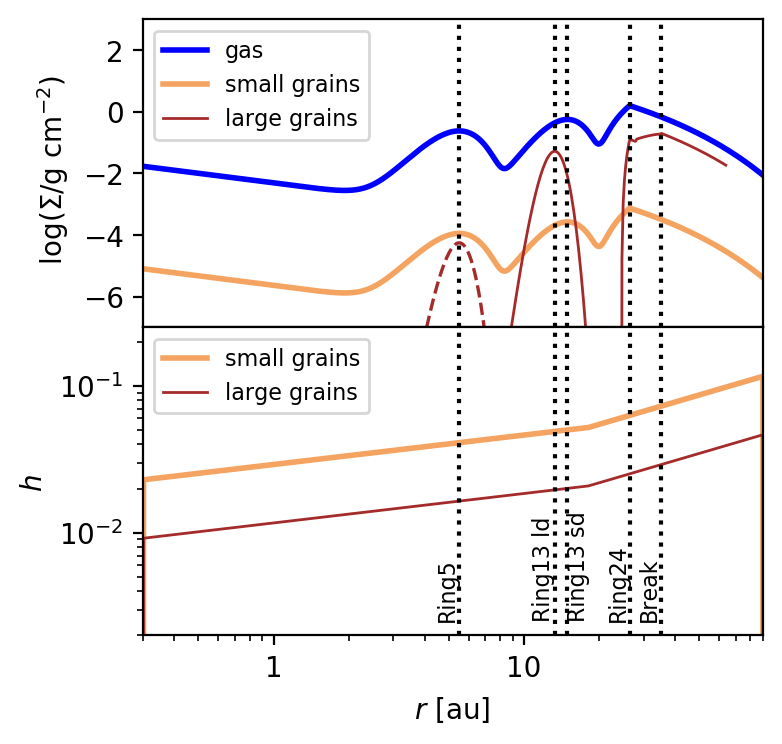
\includegraphics[width=\columnwidth]{allprofiles.png}
        \caption{{\bf Top:} surface density profiles for gas, large and small dust grains. {\bf Bottom:} Aspect ratio profile $h(r)= H(r)/r$. The dashed brown line depicts an upper limit for large dust grains within Ring5, inferred from its non-detection in ALMA data. The dotted lines crossing both panels correspond to transition radii in the parametric model.}
    \label{fig:profiles}
\end{figure}

The inner radius of the model grid was set to 0.1\,au, and the outer radius to 100\,au, which is large enough for the dust disc to be undetectable. We set the values of the inclination and disc position angle to the same as obtained from the ALMA observation in Section~\ref{sec:Observations}, such that the model has an inclination of i = 32.96\,$\degr$ and a P.A. = 77.31\,$\degr$. Finally, the distance is set to d = 71.48\,pc \citep{gaiacollaboration2020gaia}.

\section{Model results and discussion} \label{sec:results}

While certainly not unique, our parametric model is fairly successful in reproducing the available data, so it became a useful tool to discuss the real disc. The simulated images and the SED of the model are shown in Fig.~\ref{fig:images_vs_simulated} and Fig.~\ref{fig:SED} respectively.

As mentioned before, the model presented here gives a solution to a highly degenerative problem. Nevertheless, as a way to improve and obtain a rough measure of the accuracy of our model, we made one dimensional explorations of the parameter space and found uncertainties of some relevant parameters that will be useful for the discussion (see Appendix.~\ref{sec:Appendix}). We can estimate confidence intervals for the scale height at $r_\circ$= 18\,au with $H_\circ = 0.92^{+0.01}_{-0.01}$\,au, for the location of Ring5 with $r=5.2^{+0.14}_{-0.36}$\,au, and for the width of gas Ring13 of $w_\mathrm{g} = 5.18^{+0.33}_{-0.20}$\,au.

%Given those uncertainties for the width of Ring13 and the , one thought that arise is that the inner ring could be much thinner than our ALMA measurements The intrinsic error of the {\tt uvmem} correction can not be known with high accuracy, so the approximate beam may not be $1/3$ of the beam in natural weights but higher. Any change in this factor would translate to into a narrower Ring13. With a $2/5$ factor, the width of Ring13 is 2.28$\pm$0.51\,au, resulting in a marginally resolve ring. T

The simulated image at 1.65\,$\micron$ matches the radial structure of the corresponding observation to a high degree, displaying a two ringed disc, where Ring5 hides under the artificial coronagraph. The visible asymmetry in the SPHERE observations is reproduced using relatively large grains, $\sim$0.4\,$\micron$, as smaller grains did not result in such strong forward scattering. As \citet{refId0} state, the strong forward scattering that is present in the observation may indicate that the dust grains in the disc surface are relatively large, suggesting that the disc is depleted of very small grains. Alternatively, it may suggest that grains are not spherical as assumed in the calculations of opacities using Mie theory. Interestingly, the model accurately shows the shadows described by \citet{dOrazi} that are present in the SPHERE--IRDIS image.

\begin{figure}
	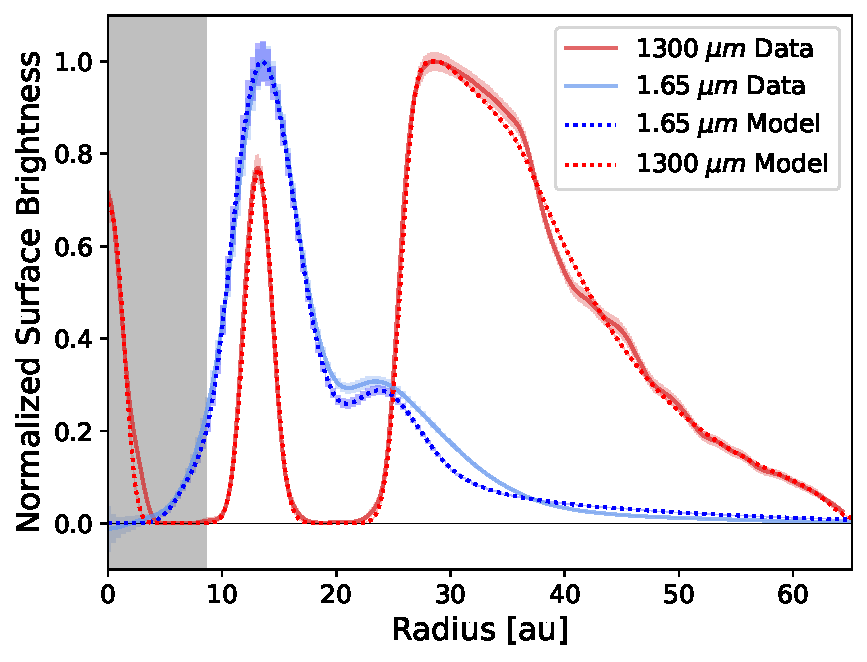
\includegraphics[width=\columnwidth]{comp_fig_all_profiles_au.pdf}
    \caption{Comparison of the surface brightness profiles extracted from the deprojected synthetic images and observed \textit{H}-band and 1.3\,mm continuum images. The grey shaded area represents the radius of the artificial coronagraph used in the simulations (i.e., $\sim0\farcs 1$, or $\sim$7.1\,au at 71.48\,pc).}
    \label{fig:radprofiles}
\end{figure}

The simulated 1.3\,mm continuum image reproduces the two observed rings: the faint Ring13 and the brighter Ring24. The introduced Ring5 is not visible in the simulated image as its predicted peak intensity is around two times the noise in the ALMA image ($\sim$1$\times10^{-7}$\,Jy\,$\mathrm{beam}^{-1}$). This gives us an upper limit for the total millimetre--sized dust mass present in Ring5 of $\sim$2$\times10^{-5}$\,M$_{\earth}$. The depletion of large dust grains in Ring5 is consistent with efficient dust trapping in Ring13. A zone of radially increasing gas pressure can entirely filter out large dust grains from inner regions, while smaller grains can be able to overcome this barrier due to their strong frictional coupling to the gas accretion flow \citep[studied in the context of planetary gaps,][]{Rice2006,Zhu2012,Weber2018}. Still, the strong depletion of large particles demands that within Ring5 dust evolution is extremely inefficient or limited, or that large particles are rapidly removed. Otherwise, the present small grains should quickly coagulate to form detectable grain sizes in the ALMA observation in Fig.~\ref{fig:images_vs_simulated} \citep{Drazkowska2019}. The central emission is also well reproduced with the inclusion of a Gaussian close ring, resulting in the observed central blob. The lack of a high NIR excess in the SED indicate that the dust in this blob must be at least bigger than 0.5\,mm (see Appendix~\ref{sec:Appendix}), but we choose to use 0.8\,mm as the lower limit for the dust population that composes this feature because this predicts a dust mass of 0.012\,M$_{\earth}$, that is in agreement with the mass estimate of \citet{Francis_2020} (0.013$\pm$0.002\,M$_{\earth}$). 

As the radial profiles obtained from the simulated images of the model closely resemble those deduced from the observations (Fig.~\ref{fig:radprofiles}), we can assume that the model provides a possible approximation of the disc structure, including the dimensions of Ring13. The FWHM of the gas in Ring13 in the RT model corresponds to $w_\mathrm{g} = 5.18^{+0.32}_{-0.20}$\,au, but the  large dust grains have to be radially converged to explain the ALMA image. Accordingly, taking the parametric model values for the large dust in Ring13, it has a FWHM of 2.00\,au, a radius of 13.22\,au, and a scale height FWHM of the millimetre-sized dust of 0.25\,au. The total dust mass of Ring13 would be about 0.7\,M$_{\earth}$. The model predictions for the millimetre-sized dust population in Ring13 are close to the measurements, with only a 0.07\,au difference in the centroid location of the ring, and a 0.46\,au difference in the width estimation. Since the scale height FWHM of the large grains in Ring13 is 0.25\,au, and that from the ALMA observation we can resolve a width of 2.46$\pm$0.40\,au (See sec.~\ref{subsec:ALMA}), the ring is 9.7$\pm$1.5 times more extended radially than vertically. Looking at the rest of the disc, in turn, our model reproduces the observations of Ring24 with peak intensity at $\sim$30\,au, and breaks at $\sim$36\,au. It contains a total dust mass of $\sim$45\,M$_{\earth}$.%, that stands under the lower limit of 60\,M$_{\earth}$ inferred by \citet{Ru_z_Rodr_guez_2019} from a previous 860\,$\micron$ continuum ALMA image. 

The observed structure may point to the existence of planet-disc interactions within this system, where a giant planet depletes its orbit of gas and dust material. A possible constellation in this scenario is, therefore, the presence of two giant planets in the disc, one planet between the star and Ring13, and one planet between Ring13 and Ring24. As \citet{Ru_z_Rodr_guez_2019} suggest, the putative planet between Ring13 and Ring24 may be a giant planet with a mass within the range of 0.3$-$1.5\,$\mathrm{M}_{\mathrm{Jup}}$. This idea is supported by the similarity to the structure around HD\,169142 which \citet{2020arXiv200711565B} reproduced by including several giant planets.

Even though the radial spread of large dust grains in Ring13 appears to be quite thin, the width in comparison to the sub-lying gas profile speaks for the presence of considerable turbulent diffusion. Following a similar ring analysis as in \citet{2018ApJ...869L..46D}, we find that the ratio between the dimensionless diffusion parameter, $D_{\rm d}$, and the dimensionless Stokes number, St, (which parameterizes the dynamical behaviour of a grain) is roughly, $D_{\rm d}/{\rm St}\approx 0.1$. The observed signal is expected to be dominated by grains of size $a\approx 0.02\,{\rm cm}$. The RT model, together with the dust-to-gas ratio of 0.05, prescribe a gas density of $\Sigma_{\rm g} \approx 0.5\,{\rm g}{\rm cm}^{-2}$ to the location of Ring13. With these values, the relevant Stokes number is approximated to be St$\approx 0.1$. This yields an estimate for the level of diffusivity of $D_{\rm d}\approx 0.01$. It further provides a value for the level of turbulent viscosity in Ring13, $\alpha_{\rm turb}\approx 0.01$, assuming the level of turbulence to be equal to the level of diffusion \citep{2007Icar..192..588Y}. We note that an observation of molecular line broadening has found no evidence for turbulent contributions, suggesting $\alpha_{\rm turb}<0.01$ \citep{Flaherty_2020}. The value inferred from our model is just within this limit. By our definition of the gas surface density profile, the value inferred for the level of turbulence is linearly proportional to the local dust-to-gas ratio. Lower values than the chosen ratio of 0.05 would, therefore, lead to an equally lower level of turbulence in the assessment. While the exact value for $\alpha_{\rm turb}$ is not well constrained, a certain level of turbulence is required to explain the radial spread of the resolved Ring13.

The observed SED is compared with the model in Fig.~\ref{fig:SED}. From the similarity with the data, we propose that there has to be a small-grain population close to the stars down to 0.3\,au, i.e. an inner disc, as it was crucial to fit the 5--10\,$\micron$ range. On the other hand, the observed central and compact signal in the ALMA observation cannot be explained with the hypothesis of thermal emission from large grains in the inner disc. Following the mass estimates in Section~\ref{sec:Observations}, the millimetre-sized dust needed reaches $\sim$18 times larger surface densities than in the gas, resulting in a large excess at 10$\,\micron$ that does not match the data. Meanwhile, the decision of employing the three-ringed structure (i.e. add Ring5 to the observed structure) relies on the fact that the SED needed a ring at a radius around 4--6\,au to have a proper fit around 10\,$\micron$, otherwise, instead of the distinct bump that is present, there would be a gap.

\section{Conclusions} \label{sec:Conclusions}

Observing the same source at different wavelengths, or employing more than one instrument, will tell different stories about the same physical phenomena. Using radiative transfer simulations let us find a common plot that may explain all this diverse results. For V4046\,Sgr, there was a missing piece for an accurate representation of the system: a thin ring of millimetre-sized dust grains at a distance of $\sim$13\,au. We presented new ALMA 1.3\,mm continuum imaging of this circumbinary disc at an unprecedented definition ($\sim0\farcs021 \, \times \, \sim0\farcs018$) were this new ring becomes visible for the first time. The new observed feature gives us some insights of the dynamics that are driving the formation of this unique morphology. Together with the analysis of SPHERE--IRDIS polarized images and a well-sampled SED, the radiative transfer modeling came as a useful tool for increasing the scope of our investigation.

The key conclusions of this multi-layered analysis are as follows.
\begin{enumerate}
  \item We report the detection of a two-ringed disc structure. The narrow ring in the 1.3\,mm continuum, has a radius of 13.15$\pm$0.26\,au and an estimated width of 2.46$\pm$0.40\,au. The location of this ring is coincident with the inner ring observed in the scattered-light image, revealing that the ring includes around 0.7\,M$_{\earth}$ millimetre-sized grains. Using the parametric model scale height FWHM value for the large grains ($H=$ 0.6\,au at 13.15\,au) we find that the ring width is roughly 4 times its estimated height. The 1.3\,mm outer ring, that starts at $\sim$24\,au and has its peak intensity at $\sim$30\,au, presents a visible break in the surface brightness at $\sim$36\,au.
  
  \item The resolved radial width of Ring13 speaks for the presence of a considerable level of turbulent viscosity.
  
  \item The central emission observed by ALMA might be by 
    
  \item We interpret the asymmetry observed with SPHERE--IRDIS at 1.65\,$\micron$ as due to strong forward-scattering, which implies that the dust population is depleted of grains smaller than $\sim$0.4\,$\micron$.
  
  \item Our parametric model, which accounts for the SED of the system, involves the existence of a sub-micron dust population close (<5\,au) to the stars, and predicts the presence of another inner ring at $\sim$5\,au, mainly consisting of small dust grains.
    
  %We also predict the existence of another thin ring at $\sim$6\,au, about 3\,au-wide and made of small dust grains, and that lies under the coronagraph of the scattered-light image. 
  %The weak central emission at 1.3\,mm could be part of this ring.
\end{enumerate}

\section*{Acknowledgements}

S.C. acknowledges support from FONDECYT grant 1171624. S.P. acknowledges support from the Joint Committee of ESO and the Government of Chile and FONDECYT grant 1191934. A.Z. acknowledges support from the FONDECYT Iniciaci\'on en investigaci\'on project number 11190837. MC acknowledges support from ANID PFCHA/DOCTORADO BECAS CHILE/2018-72190574. This paper makes use of the following ALMA data: ADS/JAO.ALMA \#2017.0.01167.S. ALMA is a partnership of ESO (representing its member states), NSF (USA) and NINS (Japan), together with NRC (Canada), MOST and ASIAA (Taiwan), and KASI (Republic of Korea), in cooperation with the Republic of Chile. The Joint ALMA Observatory is operated by ESO, AUI/NRAO and NAOJ. The National Radio Astronomy Observatory is a facility of the National Science Foundation operated under cooperative agreement by Associated Universities, Inc. This research has made use of the VizieR catalogue access tool, CDS, Strasbourg, France (DOI : 10.26093/cds/vizier). The original description of the VizieR service was published in \citet{2000A&AS..143...23O}. This research has made use of the NASA/IPAC Infrared Science Archive, which is funded by the National Aeronautics and Space Administration and operated by the California Institute of Technology.

\section*{Data Availability}

The data used in this article are presented in Fig.~\ref{fig:images_vs_simulated}. The final images can be found in FITS format in supplementary materials while the original raw data can be downloaded directly from the ALMA archive using project code 2017.1.01167.S. The SPHERE/IRDIS data can be downloaded from the ESO archive using project code 096.C-0523(A).

%%%%%%%%%%%%%%%%%%%% REFERENCES %%%%%%%%%%%%%%%%%%

% The best way to enter references is to use BibTeX:

\bibliographystyle{mnras}
\bibliography{bibtex} % if your bibtex file is called example.bib


% Alternatively you could enter them by hand, like this:
% This method is tedious and prone to error if you have lots of references
%\begin{thebibliography}{99}
%\bibitem[\protect\citeauthoryear{Author}{2012}]{Author2012}
%Author A.~N., 2013, Journal of Improbable Astronomy, 1, 1
%\bibitem[\protect\citeauthoryear{Others}{2013}]{Others2013}
%Others S., 2012, Journal of Interesting Stuff, 17, 198
%\end{thebibliography}

%%%%%%%%%%%%%%%%%%%%%%%%%%%%%%%%%%%%%%%%%%%%%%%%%%

%%%%%%%%%%%%%%%%% APPENDICES %%%%%%%%%%%%%%%%%%%%%
\appendix

\section{Parameter--space exploitation} \label{sec:Appendix}

The model presented here has many degrees of freedom and each model requires a high level of computational power and time, so a MCMC optimization or similar methods of parameter exploration are impossible to acquire. But as a way to compute a measure of goodness of fit and to try to quantify the improvements, we did a partial exploration of the parameter space. We explore $\chi^2$ space in the vicinity of the model values for the scale height at $r_\circ$, the location of Ring5, the width of the gas component of Ring13, the width of the gas part of Ring5, the width of the large dust portion of Ring13 and around the lower limit of the grain sizes in the blob. The parameter space exploration is shown in Figure~\ref{fig:chi}. Our model fits the SED and two images, so the total $\chi^2$ value for a given model is composed of the sum of the $\chi^2$ values for each of the three fits.
\begin{equation}
    \chi^2_{\mathrm{total}}=\chi^2_{\mathrm{SED}}+\chi^2_{\mathrm{ALMA}}+\chi^2_{\mathrm{SPHERE}}
\end{equation}

For the first three parameters, we find that the value of the parameter in our model is almost at a minimum in its one dimensional $\chi^2$ space, so given $\chi^2_m$ the total chi squared value for the model, the uncertainties (up and down) will be those with $\chi^2=\chi^2_m+1$. As the values are around a local minimum, we can as assume a quadratic equation for the curve fitting.

For the the other three parameters, we found that although our chosen values are close to a minimum, the geometries are more suggestive of different border conditions. These exploration allow us to support the idea of Ring5, as it is clear that the absence of it creates a great increment in the total $\chi^2$ value, but also that the ring must be quite thin. For the case of the lower limit of the central blob, it is evident that there is a threshold around 500\,$\micron$ where the SED start to deviate far away from the typical value. That point represent where the NIR excess becomes significant.

\begin{figure*}
	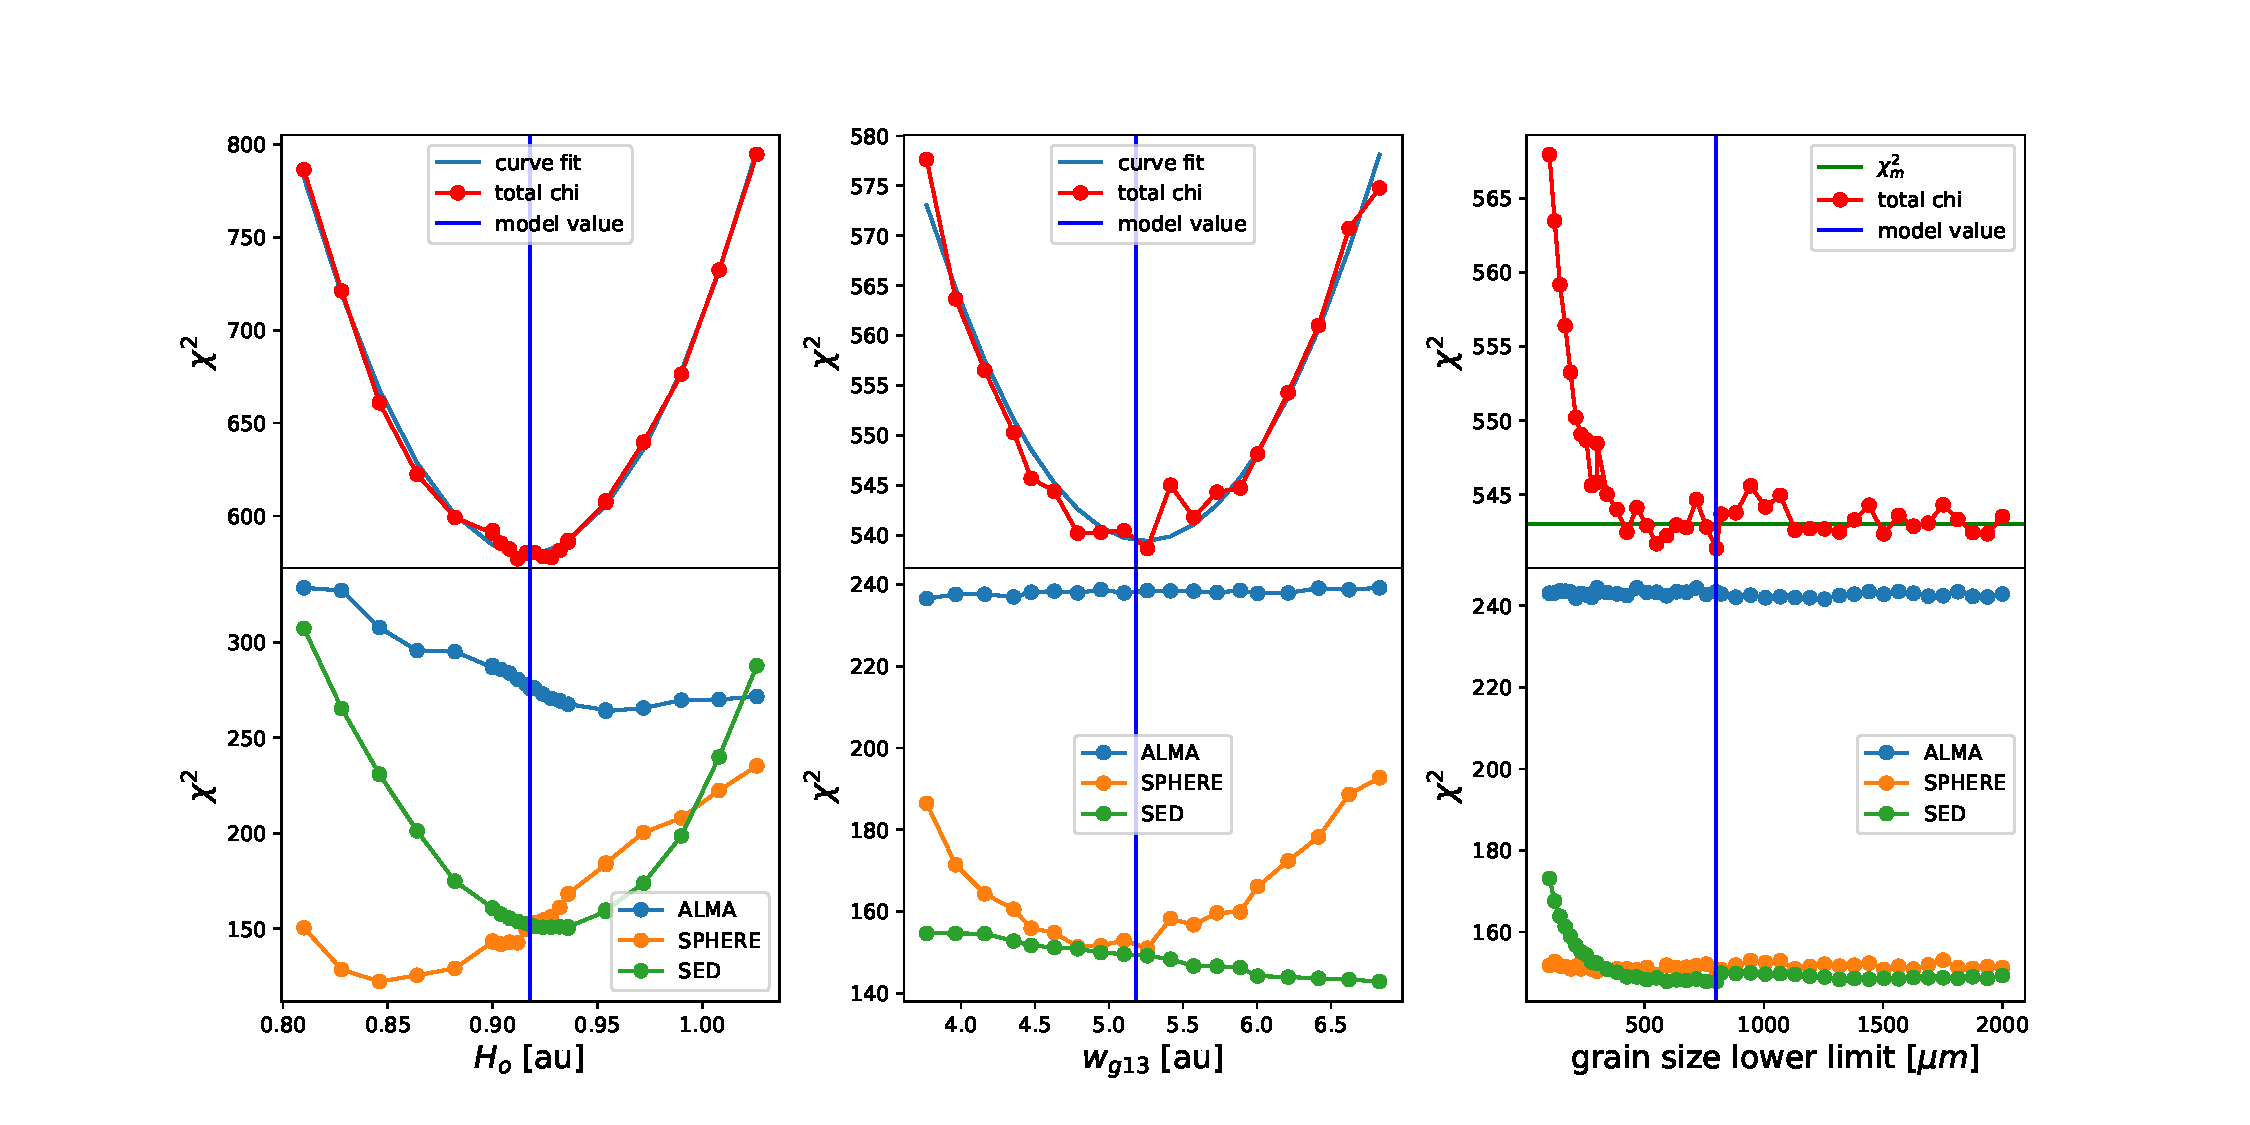
\includegraphics[width=\textwidth]{plot_chi_squared_all800.pdf}
        \caption{one dimensional explorations of the chi squared space of our parametric model. Each panel display at the bottom the $\chi^2$ values for the SED and for the two images separately, and on top the total $\chi^2$ value in terms of the parameter value. {\it Top:} scale height at $r_\circ$=18\,au, location of Ring5, width of the gas component of Ring13. {\it Bottom:} Width of the gas part of Ring5, width of the large dust section of Ring13, lower limit of the grain sizes in the blob.}
    \label{fig:chi}
\end{figure*}

%%%%%%%%%%%%%%%%%%%%%%%%%%%%%%%%%%%%%%%%%%%%%%%%%%

%%%%%%%%%%%%%%%%%%%%%%%%%%%%%%%%%%%%%%%%%%%%%%%%%%


% Don't change these lines
\bsp	% typesetting comment
\label{lastpage}
\end{document}

% End of mnras_template.tex